\thispagestyle{empty}
\chapter{Perspective : À la découverte de nouveaux virus à ADN}
{\hypersetup{linkcolor=GREYDARK}\minitoc}
\label{chap:discuss-new_viral_discovery}

\label{sec:perspective}

\section{Découvrir de nouveaux virus à ADN dans nos assemblages}

À l'exception de quelques bactéries intracellulaires aux génomes hautement dégradés, toutes les formes de vie cellulaire sont associées à des virus \citep{kristensen_new_2010, koonin_virocentric_2013}. Pourtant, selon des données récentes approximatives, moins de 1 \% de tous les virus de la biosphère sont actuellement couverts et classés \citep{geoghegan_comparative_2017}. Les techniques conventionnelles de détection et de découverte des virus, qui nécessitent une connaissance préalable des séquences génomiques virales, sont considérées comme l'une des raisons de cette vision limitée de la biosphère virale \citep{nouri_insect-specific_2018}. De papiers récents ont permis d'agrandir considérablement la diversité de virus à ARN \citep{shi_redefining_2016, wu_abundant_2020}. L'idée sous-jacente venant du fait que les virus à ARN peuvent être découverts à l'aide du séquençage métatranscriptomique en recherchant les séquences conservées d'ARN polymérase \citep{bonning_insect_2019, shi_genomes_2019, wu_abundant_2020}. Ainsi, dans leur étude, \cite{shi_redefining_2016} ont par exemple examiné le profil transcriptomique de plus de 220 espèces d'invertébrés échantillonnées dans neuf phylums animaux. Ils ont alors pu  décrire 1,445 virus à ARN, dont certains sont suffisamment divergents pour constituer de nouvelles familles comme celles des \textit{Chuviridae} par exemple. 

Ainsi, le taux de découverte de virus est largement déterminé par la disponibilité accrue du séquençage à haut débit. Cependant, l'assemblage de lectures courtes en contigs, en particulier, reste coûteux en termes de calcul, ce qui limite l'étendue des échantillons analysés. Des stratégies alternatives commencent donc à émerger visant à découvrir de nouveaux virus à moindre coût, comme celle de la base de donnée \textit{Serratus}. Cette base de donnée réanalyse toutes les données de séquençage, d'ARN-seq, de métagénomique, et de métatranscriptomique  dans les archives (SRA) de NCBI (plus de 10 000 000 de gigaoctets de données !). L'idée est donc de se baser sur l'alignement de reads qui est nettement moins coûteux que l'assemblage et qui permet le traitement de grands ensembles de données \citep{edgar_petabase-scale_2022}.

L'exploration de la virosphère d'ADN, en revanche, peut être une procédure plus difficile en raison du fait qu'aucun gène n'est conservé universellement chez ces virus \citep{iranzo_double-stranded_2016}. Il existe cependant des gènes cœurs conservés au niveau des classes de virus. En partant du principe qu'un génome viral à ADN doit être séquencé en même temps que l'ADN de l'espèce cible lors du séquençage (dépend néanmoins de sa densité relative dans les tissus), il est donc possible d'exploiter directement les données génomiques telles que les assemblages ou les lectures brutes et trouver par homologie de séquences des virus. 

Aussi, plusieurs méthodes s'offrent à nous. Une première consiste tout comme exploré dans \hyperref[sec:chap2]{chapitre 2}, à analyser les contigs à la recherche d'homologies de séquences convaincantes avec des protéines virales.

Une perspective afin d'améliorer l'efficacité de la recherche de nouveaux virus à ADN à l'échelle métagénomique serait de systématiquement analyser les assemblages génomiques avec une approche d'alignement de type BlastX avec en query les contigs, et en base de données toutes les protéines virales connues. À ce propos, un nouveau module a récemment vu le jour dans l'équipe qui développe Mmseqs2 (Mmseqs taxonomy), dont la fonction est spécifiquement d'assigner un niveau taxonomique rapide à plusieurs milliers de contigs. Le principe repose alors sur un système de vote qui assigne une taxonomie à un contig selon la distribution des taxonomies associées à chacun des hits convaincants le long de ce dernier \citep{mirdita_fast_2021}. Cette approche, combinée à celle que j'ai développée lors du \hyperref[sec:chap2]{chapitre 2} dans lequel je tague les contigs selon qu'ils appartiennent probablement au génome nucléaire ou à des entités libres, pourrait ainsi permettre de proposer une méthode de détection robuste de nouveaux contigs viraux, voire de génomes entiers si les couvertures de séquençages sont suffisamment grandes. À ce propos, si nous regardons dans les données générées à partir de l'assemblage de 124 génomes d'Hyménoptères, j'ai pu observer 1419 scaffolds présentant un ou plusieurs hits convaincants avec un score d'identité de moins de 90\% avec des protéines virales (Table\ref{table:Free-living_viruses}). Ces résultats devront être exploités, car ils nous permettront très probablement de découvrir de nombreux nouveaux virus chez au moins 62 Hyménoptères (Table\ref{table:Free-living_viruses}). Les familles virales les plus représentées sont les \textit{Iridoviridae} (164 scaffolds), \textit{Baculoviridae} {135}, et \textit{Phycodnaviridae} (135) (Table\ref{table:Free-living_viruses}). Ainsi, par exemple, nous pouvons voir que parmi 129 scaffolds chez 37 espèces d'Hyménoptères, 264 hits avec des protéines de poxvirus sont retrouvés (dont 200 sont associées à des \textit{Entomopoxvirinae}). Ces séquences peuvent alors constituer de nouveaux virus provenant de cette sous-famille virale bien connue pour infecter les insectes \citep{theze_new_2013}.


% \usepackage{array}
% \usepackage{graphicx}
% \usepackage{booktabs}

% \usepackage{graphicx}
% \usepackage{booktabs}


\begin{table}[!htbp]
\centering
\resizebox{\linewidth}{!}{%
\begin{tabular}{l|lll} 
\toprule
\textbf{Famille virale putative} & \textbf{Nb Scaffolds} & \textbf{Nb hits} & \textbf{Nb espèces HyméŽnoptères} \\ 
\hline
\textbf{\textit{Iridoviridae}} & 164 & 516 & 33 \\
\textbf{\textit{Baculoviridae}} & 135 & 211 & 36 \\
\textbf{\textit{Phycodnaviridae}} & 135 & 258 & 34 \\
\textbf{\textit{Ascoviridae}} & 134 & 238 & 29 \\
\textbf{\textit{Poxviridae}} & 129 & 264 & 37 \\
\textbf{\textit{Nudiviridae}} & 108 & 139 & 33 \\
\textbf{\textit{Mimiviridae}} & 97 & 176 & 27 \\
\textbf{Filamentoviridae} & 84 & 147 & 25 \\
\textbf{\textit{Caulimoviridae}} & 78 & 78 & 26 \\
\textbf{\textit{Marseilleviridae}} & 69 & 153 & 21 \\
\textbf{\textit{Hytrosaviridae}} & 61 & 88 & 20 \\
\textbf{\textit{Asfarviridae}} & 35 & 50 & 10 \\
\textbf{\textit{Parvoviridae}} & 29 & 34 & 11 \\
\textbf{\textit{Herpesviridae}} & 28 & 32 & 15 \\
\textbf{\textit{Nimaviridae}} & 27 & 32 & 14 \\
\textbf{\textit{Alloherpesviridae}} & 21 & 23 & 10 \\
\textbf{\textit{Polydnaviridae}} & 21 & 23 & 10 \\
\textbf{AmFV-like} & 10 & 29 & 47 \\
\textbf{\textit{Lavidaviridae}} & 9 & 9 & 6 \\
\textbf{IVSPERs} & 8 & 8 & 8 \\
\textbf{\textit{Adenoviridae}} & 7 & 8 & 6 \\
\textbf{\textit{Bidnaviridae}} & 5 & 5 & 3 \\
\textbf{\textit{Circoviridae}} & 5 & 7 & 1 \\
\textbf{\textit{Genomoviridae}} & 5 & 8 & 2 \\
\textbf{\textit{Malacoherpesviridae}} & 5 & 5 & 5 \\
\textbf{\textit{Geminiviridae}} & 4 & 7 & 2 \\
\textbf{\textit{Lipothrixviridae}} & 3 & 3 & 2 \\
\textbf{\textit{Smacoviridae}} & 2 & 2 & 1 \\
\textbf{\textit{Alphasatellitidae}} & 1 & 1 & 1 \\
\textbf{Total} & 1419 & 2554 & 62 \\
\bottomrule
\end{tabular}
}
\caption[Perspective:Classification des scaffolds exogènes provenant du chapitre1]{Tableau classant tous les scaffolds provenant probablement de sources virales exogènes (classés F ou X) de l'analyse du \hyperref[sec:chap1]{chapitre 1} parmi 124 assemblages d'Hyménoptères et dont le pourcentage d'identité protéique est inférieur à 90\%.}
\label{table:Free-living_viruses}
\end{table}

\subsection{Exemple de la présence d'un nouveau virus de la sous-famille des \textit{Entomopovirinae} chez \textit{Encarsia formosa}}

Ainsi, en prenant un scaffold parmi ces 129 (le scaffold\_187 chez l'espèce endoparasitoïde \textit{Encarsia formosa}), nous parvenons à observer que ce scaffold provient très probablement d'un virus libre apparenté à un entomopoxvirus.

La démarche pour arriver à cette conclusion comprend plusieurs étapes que je discute par la suite, en proposant des pistes d'améliorations :

\begin{itemize}

    \item (1) Taguer les scaffolds ayant des signatures de scaffolds libres (c-à-d provenant d'entités génomiques non intégrées au génome nucléaire de l'espèce séquencée). Ici plusieurs arguments nous permettent de privilégier l'hypothèse qu'il s'agit d'un scaffold libre : 
    
    \begin{itemize}
       \item  \textbf{La couverture et le contenu en GC}- La couverture moyenne de ce scaffold est de 19X alors que la moyenne des couvertures des scaffolds qui contiennent des BUSCOs est de 33x, de plus le contenu en G+C est également significativement différent pour le scaffold (16.63\%) comparé à la moyenne des scaffold BUSCOs (33\%). La couverture et le GC sont \textit{a priori} propre à chaque entité séquencée, ces données confortent donc dans l'idée qu'il s'agit de scaffolds appartenant à des entités différentes de celles du génome de \textit{E.formosa}. 
       
       \item \textbf{Densité en ORFs}- Puisque les virus présentent des densités en gènes plus fortes comparés à des organismes eucaryotes \citep{mahmoudabadi_comprehensive_2018}, nous pouvons utiliser cette caractéristique comme indice pour discriminer des scaffolds viraux. Ainsi, lorsqu'on prédit des ORFs le long des scaffolds candidats, nous retrouvons 36 ORFs, dont la taille cumulée est de 31,373 pb soit 31,373/33,649 = 93.34\% de la taille des scaffolds, donc une densité forte et comparable à ce que nous pouvons observer chez les Filamentoviridae ou d'autres poxvirus \citep{zhao_genome_2011}. 
       
       \item \textbf{Absence de gènes eucaryotes}- Enfin, il est attendu que peu, voire aucune homologie avec des séquences eucaryotes ne soit retrouvée à l'intérieur de ce scaffold (tout du moins bien moins que le nombre d'homologie avec des séquences virales), car il est en effet bien connu que les génomes à grand génome ADNdb capturent régulièrement des gènes eucaryotes \citep{irwin_systematic_2022}. Ici par exemple, aucun ORF viral prédit n'a présenté d'homologie avec des séquences eucaryotes.  
       
       \end{itemize}
 
    \item (2) Inférer tous les ORFs possibles à l'intérieur de ce scaffold (Table\ref{table:Free-living_viruses}) (ici avec ORFfinder online, params : min50pb, ATG only) (comme nous le voyons dans le \hyperref[sec:chap2]{chapitre 2} il est toujours préférable de croiser la prédiction de plusieurs logiciels prédicteurs d'ORFs).

\begin{figure}[!htbp]
 \centering
  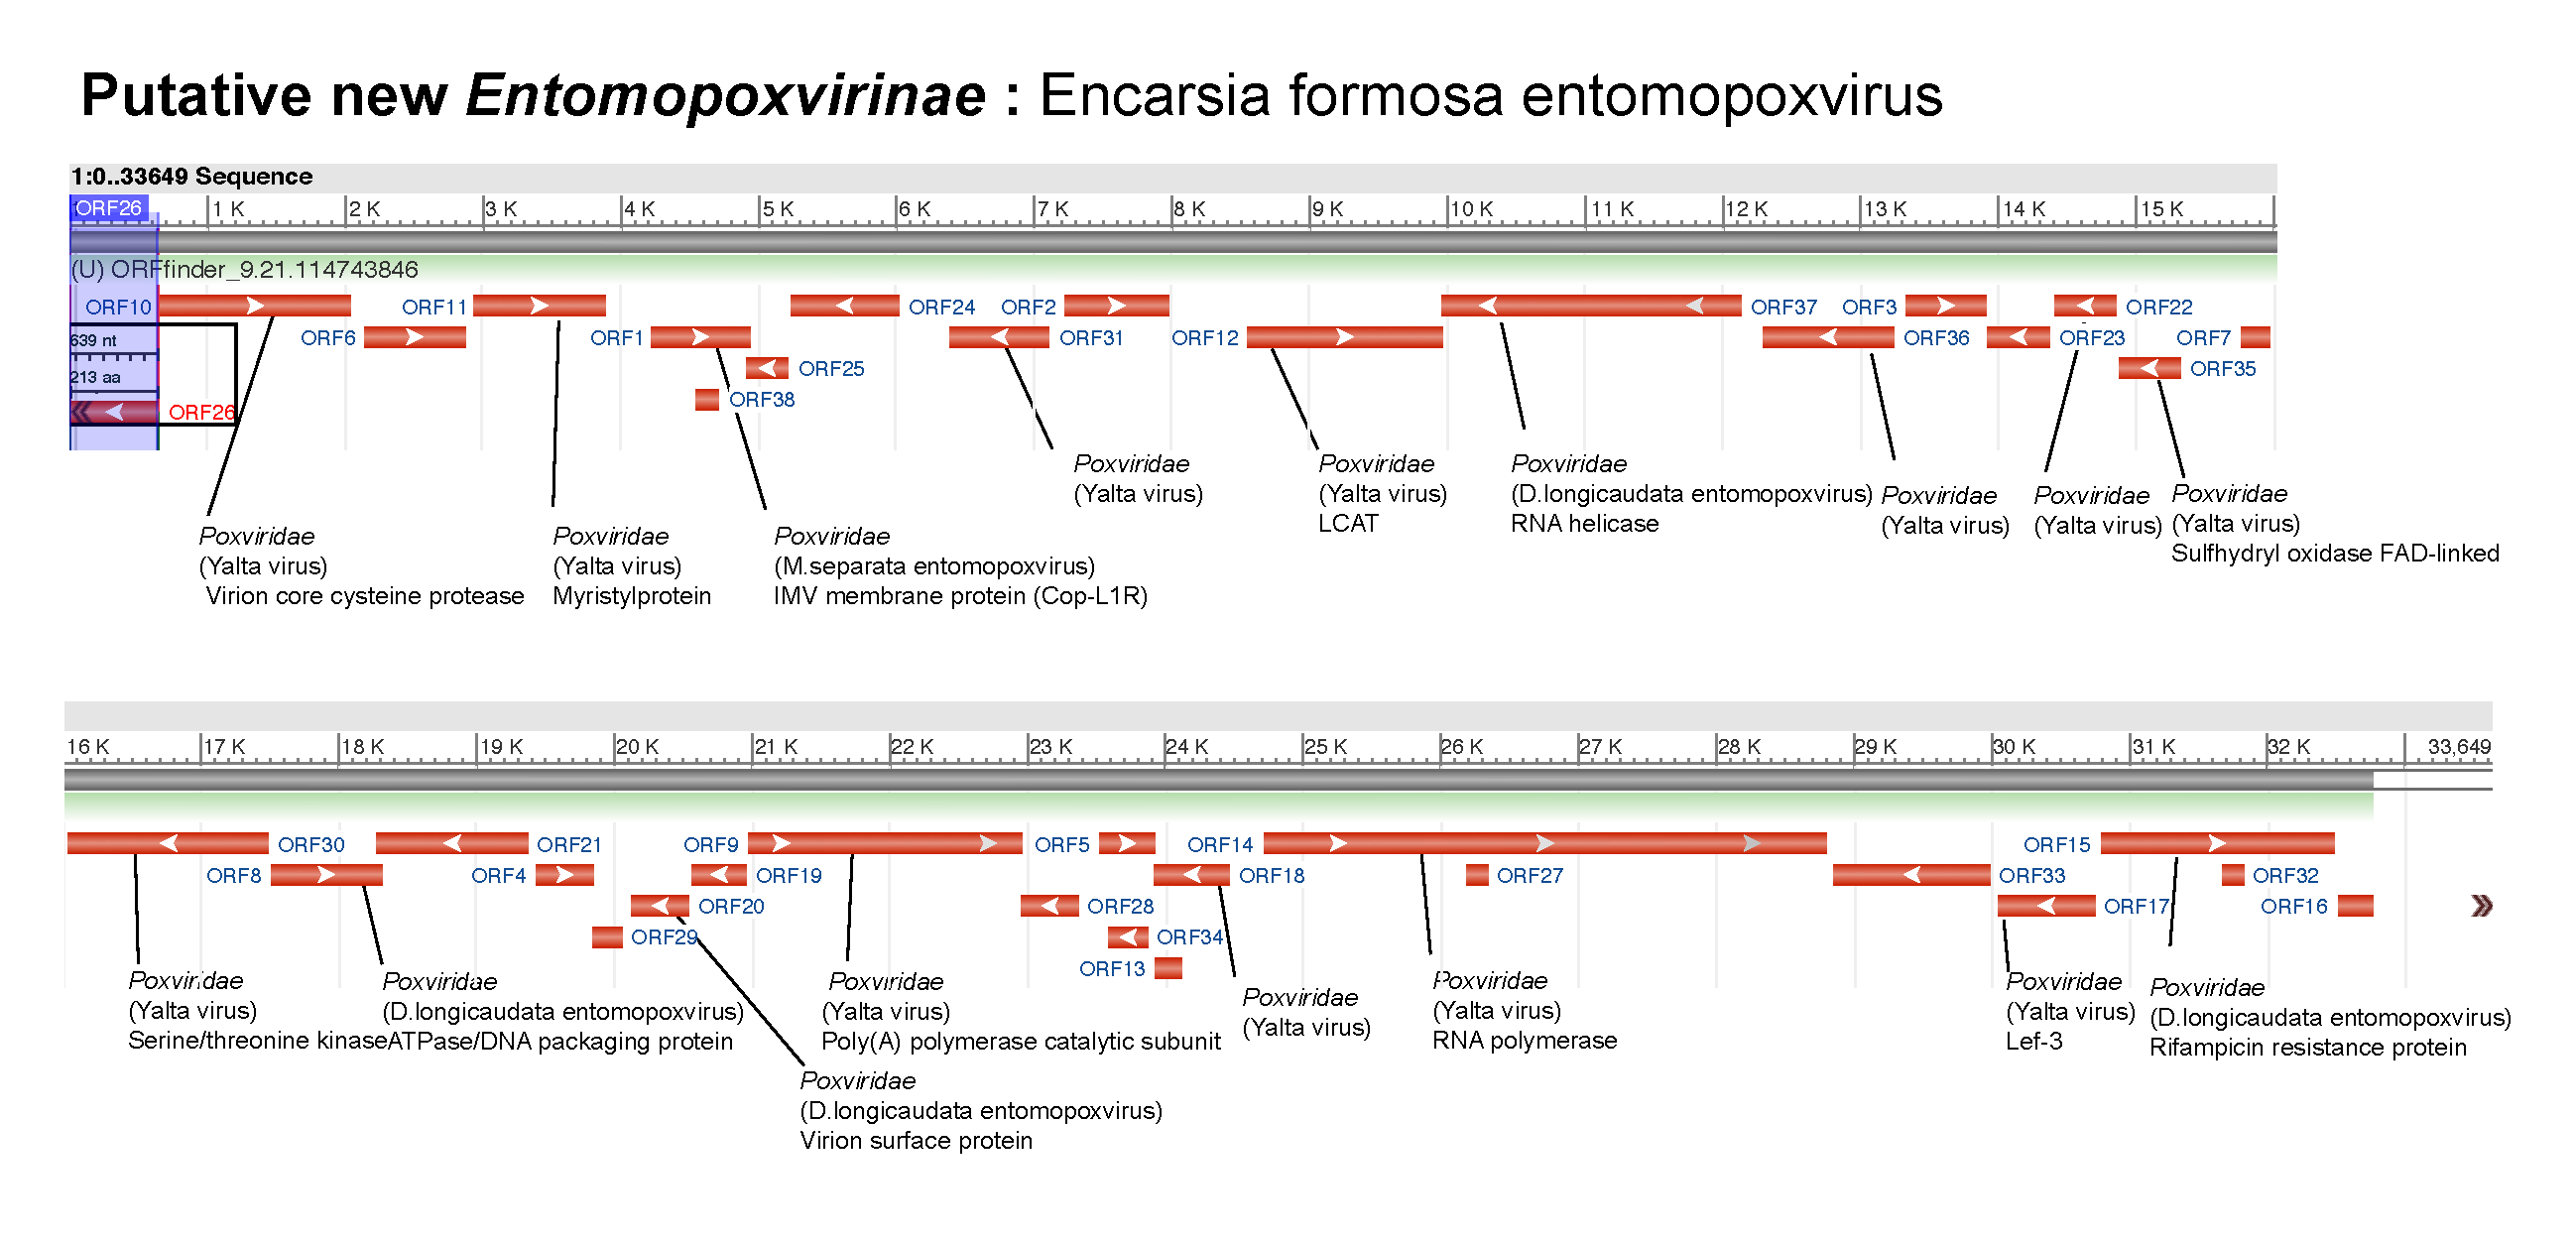
\includegraphics[width=\linewidth,height=\textheight,keepaspectratio]{PhD-master/figures/Eformosa_entomopoxvirus_scaffold.png}
\caption[Perspective:ORFs prédits le long du scaffold\_187 chez \textit{E. formosa}]{\textbf{ORFs prédits le long du scaffold\_187 chez \textit{E. formosa}.}}
\label{figure:Eformosa_entomopoxvirus_scaffold}
\end{figure}

 \item (3) Rechercher de l'homologie de séquence entre ces ORFs prédits et des protéines virales dans une base de donnée généraliste (ici NR). Ici sur 36 ORFs prédits, nous retrouvons des homologies convaincantes (bit score $>$= 50) avec tout de même 17 ORFs tous provenant d'entomopoxvirus (Table\ref{figure:Eformosa_entomopoxvirus_scaffold}). 

 \item (4) Effectuer un alignement protéique pour chacun des ORFs avec les protéines de la base de donnée ayant obtenu un hit. 

 \item (5) Concaténer chaque alignement en une seule super-matrice protéique puis inférer la phylogénie des espèces virales. Cette phylogénie est un moyen robuste d'assigner phylogénétiquement un rang taxonomique à l'échelle de la famille et surtout d'inférer l'espèce à qui appartient les scaffolds candidats. Dans notre cas, nous observons dans la phylogénie des espèces virales que la branche du virus \textit{E. formosa} se branche très clairement au sein du clade des \textit{Entomopoxvirinae} et plus particulièrement proche du Yalta virus connu pour infecter \textit{Drosophila melanogaster} \citep{wallace_discovery_2021} (le seul poxvirus connu à ce jour chez les Diptères) (\figurename{\ref{figure:Poxvirus_partition.tab.treefile}}). 
 
 \begin{figure}[!htbp]
 \centering
  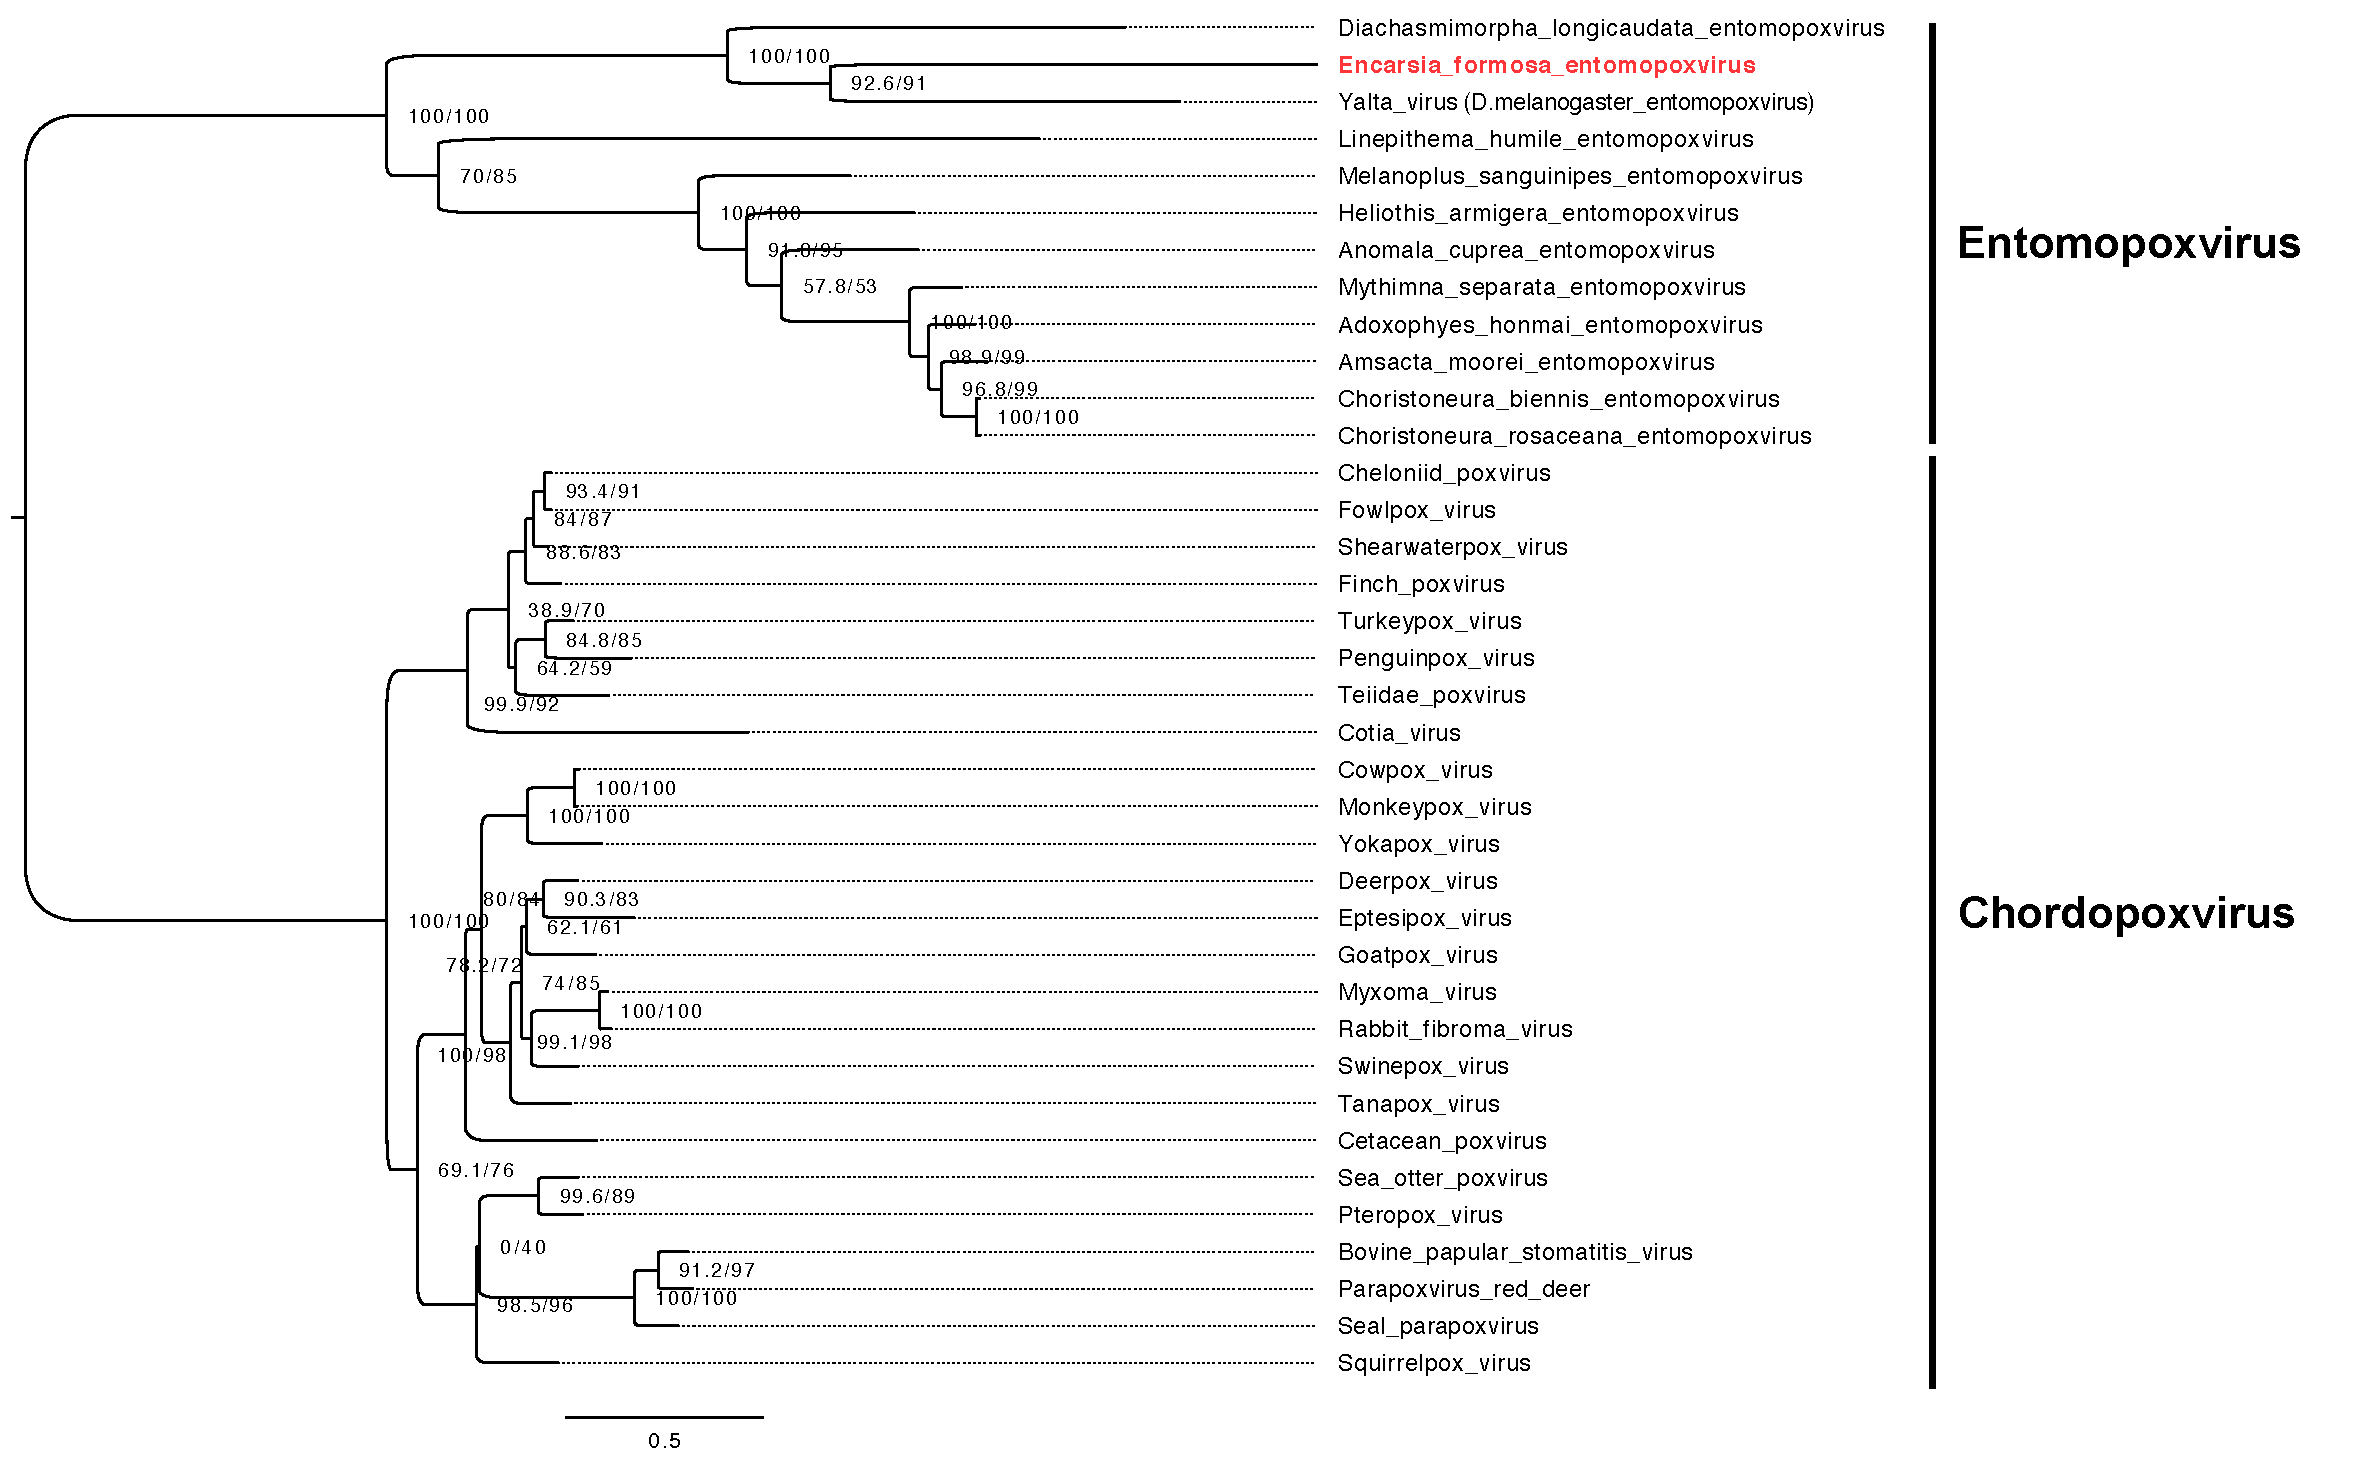
\includegraphics[width=\linewidth,height=\textheight,keepaspectratio]{PhD-master/figures/Poxvirus_partition.tab.treefile.pdf}
\caption[Perspective:Phylogénie des espèces de Poxvirus incluant \textit{E.formosa} entomopoxvirus]{\textbf{Phylogénie des espèces de Poxvirus}. La phylogénie a été inférée avec Iqtree2 (modèle partitionné, -m MFP -alrt 1000  -bb 1000 -bnni) et se base sur l'alignement protéique de 36 ORFs viraux ayant eu une homologie avec un ORF prédit dans le scaffold\_187 de l'espèce \textit{E. formosa}. Les espèces de virus ont été sélectionnées à la main. La feuille qui correspond à l'information phylogénétique provenant des 36 ORFS de \textit{E. formosa} est en rouge}
\label{figure:Poxvirus_partition.tab.treefile}
\end{figure}


\end{itemize}

Bien évidemment, il s'agit ici d'un seul exemple, mais son automatisation à l'ensemble des scaffolds et espèces virales concernées serait une tâche stimulante. D'autant que divers points d'améliorations sont à prendre en compte :\\

\textbf{Les pistes d'améliorations}

\begin{itemize}
    \item Plusieurs scaffolds viraux peuvent appartenir à une même espèce virale (dans notre exemple chez \textit{E. formosa}, le scaffold est loin d'être de la taille attendue pour un scaffold de \textit{Poxviridae} (ici de 33,649pb alors que la taille des génomes de Poxvirus est entre 130,000pb et 360,000pb \citep{hughes_evolutionary_2010}. Ainsi, parvenir à associer plusieurs scaffolds au sein de la même espèce pourrait être réalisé en partant du principe que plusieurs scaffolds assignés à une même entité taxonomique virale (même espèce ou famille par exemple) fasse effectivement partie du même génome viral.

    \item Puisqu'il s'agit d'une analyse à grande échelle, une attention toute particulière doit être apportée dans l'écriture d'un algorithme capable d'échantillonner efficacement des espèces virales. En effet, pour certaines familles virales, le nombre d'espèces séquencées peut être si important que leur ajout donnerait lieu à des matrices trop grandes pour être calculées en un temps raisonnable. Aussi, il sera judicieux de réfléchir à un algorithme permettant à la fois de choisir les espèces virales éloignées, et espèces proches pour rendre compte de la  diversité virale en question. 
    
    \item Une limite apparaitra  lorsque les ORFs étudiés sont trop petits et présentent un seul ou très peu d'ORFs avec des homologies virales. Ce genre de cas sera compliqué à analyser, car le placement de ces virus dépendra d'un seul gène. Ainsi, si on s'intéresse par exemple au tableau \ref{table:Free-living_viruses}, nous pouvons voir qu'il existe 8 scaffolds présents chez 8 espèces virales qui présentent des homologies convaincantes avec des ORFs d'IVSPERs. Ce simple ORF chez les 8 espèces n'est pas suffisant pour montrer qu'il existe un virus apparenté aux IVSPERs préalablement décrit chez l'espèce \textit{H. dydimator}, qui provient par ailleurs d'un virus inconnu (ichnovirus). Dans la même veine, nous retrouvons chez de l'espèce de fourmis \textit{Cataglyphis\_hispanica} un seul ORF parmi 4 prédits présentant une homologie avec des séquences de \textit{Cruciviridae}. Un moyen de tout de même appuyer l'hypothèse d'un scaffold viral peut-être, comme nous l'avons proposé, d'observer une densité en ORF plus élevée qu'attendue pour une séquence eucaryote (ici, elle est de 85\%). Un autre argument peut être également de comparer la taille du génome et le contenu en ORF attendu chez les virus déjà connus. Aussi, dans ce cas précis, la taille attendue des génomes chez les virus à ADNsb va de 2,000 à 6,000pb \citep{campillo-balderas_viral_2015}, ce qui coïncide avec la taille du scaffold rencontrée chez \textit{Cataglyphis\_hispanica} (3,588pb). 
  
    \item Enfin, examiner à cette échelle à la main chaque phylogénie afin d'inférer un rang taxonomique pour chaque scaffold est impossible. C'est pourquoi le développement d'un algorithme permettant de lire les phylogénies et de sortir la taxonomie des séquences les plus proches sera indispensable, en prenant en compte les scores de bootstrap afin de collapser les nœuds peu soutenus. 
    
\end{itemize}

D'autres approches plus généralistes, mais qui ne permettent pas de prendre en compte la phylogénie, pourraient également s'inspirer de l'approche développée par Serratus \citep{edgar_petabase-scale_2022} principalement pour les virus à ARN. L'idée étant d'aligner des reads provenant de la métagénomique et de trouver des alignements convaincants avec des bases de données nucléotidiques virales également. Une limitation possible à ce genre d'approche proviendrait du fait qu'il est envisageable qu'une partie des nouveaux candidats viraux proviennent de portions génomiques virales endogénisées. Cependant, le phénomène d'endogénisation étant relativement rare, cette limitation devrait être anecdotique (seulement 1\% dans le jeu de donnée de Serratus sont étiquetés comme étant des EVEs par exemple \citep{edgar_petabase-scale_2022}.\\


%

%inspi de https://www.sciencedirect.com/science/article/pii/S1879625711000460

%\subsubsection{\textbf{Discovery of new free-living viruses in Hymenoptera genomes}}

%s'inspirer de https://repository.upenn.edu/cgi/viewcontent.cgi?article=6008context=edissertations 

%Les virus ont été découverts à la fin du 19ème siècle en tant que comme des pathogènes végétaux et animaux particuliers qui étaient assez petits assez petits pour passer les filtres bactériens. Depuis lors, les développements Depuis lors, les développements en virologie et en génomique ont complètement modifié le concept de virus. Nous réalisons maintenant que les virus sont omniprésents et extrêmement abondants, à la fois en termes de infectant toutes les formes de vie cellulaire connues et étant présents dans tous les environnements explorés. En fait, les virus semblent être les entités biologiques les plus abondantes de la planète, dépassant considérablement le nombre de cellules dans la plupart des habitats dans la plupart des habitats bien étudiés [1,2,3]. 

%Currently we lack a comprehensive view of the virosphere present in arthropods, which can thus in the kind of homology-based analysis as ours very strongly limit the discovery of EVEs if homologs are not present in databases, as is the case in Hyposoter dydimator for exemple in which an unknown ichnovirus has integrated and allows for polydnavirus formation (Volkoff et al 2010). Recent data suggest that currently less than 1\% of the total universe of viruses in the biosphere is covered and classified (Geoghegan et al 2017), and traditional methods of virus detection and discovery, which require prior knowledge of viral genomic sequences, are considered one of the causes of this restricted view of the biosphere (ShahidehNouri et al 2018).

%So far, viruses associated with insect pests have been described using classical approaches and metagenomic analyses (Liu et al 2011). Viruses belonging to Baculoviridae, Parvoviridae, Flaviviridae, Ascoviridae, Togaviridae, Bunyavirales, and Rhabdoviridae have thus been most commonly associated with insects (AsgariS et al 2010), but many new insect viruses have been discovered by metagenomic or transcriptomic approaches (Nouri et al, 2018, Mang Shi et al 2016). Arthropods thus contain viruses that are at the base of major virus groups, including vertebrate-specific arenaviruses, filoviruses, hantaviruses, influenza viruses, lyssaviruses, and paramyxoviruses (Ci-Xiu Li, et al 2015), or even Parvoviruses (François S et al 2016). 

%Since our analysis also allows us to characterize scaffolds from free viruses (F and X annotated scaffolds), we were also able to characterize the presence of new viruses interacting with the Hymenoptera species thanks to the homology of their genes with genes in the databases (a particular precaution must nevertheless be made on the possible aspect due to a contamination). Thus, we characterized a total of X new viruses. Interestingly, this also allowed us to enrich the number of potential viruses of the LbFV-like virus family and AmFV since until now only the genome of Leptopilina boulardi Filamentous Virus and Apis meliffera Filamentous Virus were known (D. Lepetit, et al., 2016 and Ulrike Hartman et al., 2015). 

%see Ward Deboutte et al 2020 for hymenoptera virus diversity.see Ward Deboutte et al 2020 for hymenoptera virus diversity.




